\chapter{Calcul des matrices source-récepteur par un modèle lagrangien adjoint}

L'étude de cas sur l'expérience FFT07 présentée dans le Chapitre 3 a montré que la charge de calcul de la procédure d'estimation du terme source est en grande majorité focalisée sur le calcul de la matrice source-récepteur. Cette étape nécessite une quantité d'appels au modèle de dispersion égale au nombre de particules échantillonnées par itération multiplié par le nombre d'itérations, soit en pratique 1000 instances dans le cas de FFT07. \\

Si pour les cas les plus simples il est possible de se limiter à des modèles de dispersion suffisamment rapides, la situation change dès qu'il s'agit de considérer un contexte plus élaboré, avec des outils de calculs permettant certes une meilleure représentation des phénomènes de dispersion, mais dont l'exécution devient bien plus coûteuse en termes d'implémentation et de temps de calcul. \\

L'objet de ce chapitre est ainsi de présenter une façon d'optimiser le calcul des matrices source-récepteur lorsque celui-ci doit faire appel à un code de dispersion plus complexe que le modèle à bouffées gaussiennes précédemment évoqué. La présentation de cet outil de calcul constituera la première partie de ce chapitre, avec notamment une explication de son fonctionnement, puis une présentation de son intégration optimale à la chaîne de calcul et d'estimation existante. La suite du chapitre se concentrera sur les aspects pratiques autour de la mise en application de cette méthodologie améliorée, avec la présentation des résultats sur plusieurs cas-tests de simulation.


\section{Le code de calcul PMSS}

\subsection{L'approche lagrangienne de la dispersion atmosphérique}
\label{part_lagrangian}

Pour les modèles dits eulériens, la résolution du problème de la dispersion d'un polluant dans l'atmosphère passe par la construction d'un maillage sur le domaine étudié, afin de pouvoir observer l'évolution des concentrations du polluant porté par les mouvements de l'air. 

Le point de vue lagrangien est différent: il s'agit ici de résoudre un système d'équations dans un repère lié au déplacement de la masse d'air contenant le polluant. Pour cela, on représente le panache sous la forme d'un ensemble de \textit{particules lagrangiennes}\footnote{Afin d'éviter toute confusion avec les particules statistiques dont il est fait référence dans le cadre de l'algorithme AMIS, nous utiliserons la dénomination  de \textit{particule lagrangienne} abréviée par PL dans la suite du texte. Nous conservons le terme de \textit{particule} pour désigner les échantillons issus de l'AMIS.}, chacune étant porteuse d'une masse élémentaire du polluant considéré. Le principe d'un modèle lagrangien consiste ainsi à étudier les trajectoires de ces éléments discrets dans le domaine au fil du temps.

Le fait de modéliser le panache par un ensemble de PL permet de tenir compte de la nature stochastique de leur déplacement, qui traduit la variabilité inhérente aux processus de turbulences auxquels est soumis le panache: on parle d'ailleurs plus précisément de \textit{modèle lagrangien stochastique}. On va ainsi travailler sur une équation de transport portant sur la densité de probabilité associée à chaque trajectoire. Plus formellement, d'après \cite{Flesch1995}, la formulation classique régissant un modèle de dispersion lagrangien se présente sous la forme d'une équation de Langevin, qui s'écrit: 

\begin{equation}
	\begin{split}
		du_i &= a_i(\Vecx, \Vecu, t)dt + b_{i,j}(\Vecx, \Vecu, t)d\xi_j  \\
		dx_i &= u_i dt = (\bar{u}_i + U_i)dt
	\end{split}
	\label{eq_langevin}
\end{equation}
où:
 \begin{itemize}
	\item $\Vecx = (x, y, z)$ est la position de la PL  définie par un repère spécifique: $x$ suit l'axe du vent, $y$ suit l'axe perpendiculaire au vent, et $z$ désigne l'élévation verticale classique. 
	\item $\Vecu$ est la vitesse d'écoulement à laquelle est soumise la PL: $\Vecu = (u, v, w)$ où les composantes respectives de ce vecteur suivent les mêmes axes que $\Vecx$.
	\item $a_i$ et $b_{i,j}$ sont des fonctions spécifiques de $(\Vecx, \Vecu, t)$ respectivement appelées \textit{drift term} et \textit{random forcing}.
	\item $d\xi_j$ est un incrément aléatoire suivant une distribution gaussienne de moyenne nulle et de variance $dt$.
	\item $\bar{u}_i$ représente le vent moyen et $U_i$ sa composante stochastique.
	
\end{itemize}

L'expression des fonctions $a_i$ et $b_{i,j}$ varie selon les hypothèses que l'on se fixe sur la nature de la turbulence: une présentation plus détaillée de leur calcul est disponible dans \cite{Wilson1996}. Une fois que ceux-ci sont définis,l'équation \eqref{eq_langevin} est discrétisée et sa résolution permet de calculer un ensemble de trajectoires de PL émanant d'une source dont les paramètres sont connus. Les concentrations volumiques moyennes simulées sont alors obtenues par la somme des particules présentes dans un volume élémentaire $d\Vecx$ autour du point d'observation $\Vecx$ durant un certain temps de résidence. En d'autres termes, on peut écrire la concentration moyenne au point $\Vecx$ et à l'instant $t$ comme étant : 

\begin{equation}
	C(\Vecx, t) = \int _{-\infty}^{t} \int_{V} S(\Vecx',t')p(\Vecx, t | \Vecx', t')d\Vecx'dt
	\label{eq_c_moyen_lagrangien}
\end{equation}
où $V$ est le volume défini par le domaine d'étude, $S(\Vecx',t')$ est la distribution de la source, et $p(\Vecx, t | \Vecx', t')$ est la densité de probabilité sur la position $\Vecx$ et l'instant $t$ des PL de position initiale $\Vecx'$ à l'instant $t'$. \\

\begin{figure}
	\centering
	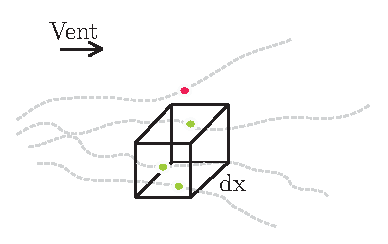
\includegraphics[width=0.65\textwidth]{lagrangian_ok}
	\caption{Principe du modèle lagrangien: la concentration en $\Vecx$ s'obtient par la somme des PL (en vert) traversant le volume élémentaire $d\Vecx$ durant un certain temps de résidence.}
	\label{fig_schema_lagrangien}
\end{figure}

Afin de calculer le champ d'écoulement auquel sont soumises les PL, plusieurs méthodes sont disponibles. Il est par exemple possible de résoudre les équations de la mécanique des fluides via un outil de simulation de type CFD, ce qui permet une modélisation fine des phénomènes physiques mis en jeu. Une autre possibilité consiste à avoir recours à une simulation dite \textit{CFD simplifiée}, où le champ de vent est interpolé à partir des mesures d'une ou plusieurs stations météorologiques tout en prenant en compte la topographie du terrain. C'est cette dernière approche qui est employée dans les outils de calcul du CEA et d'ARIA Technologies, et que nous présentons dans le chapitre suivant. \\

\subsection{La chaîne de calcul SWIFT-SPRAY}

L'outil \textit{Parallel Micro-SWIFT-SPRAY} (PMSS) est une chaîne de calcul constituée de deux éléments distincts: un outil de CFD simplifiée (SWIFT) et un modèle de dispersion lagrangien stochastique (SPRAY). Il est généralement appliqué dans des études à petite échelle (par exemple, au niveau d'un quartier), mais grâce à sa version parallèle, il a récemment été utilisé sur des domaines plus grands, à l'exemple du cas AirCity (REF) où le modèle a été exécuté sur l'ensemble de la ville de Paris.\\

\subsubsection{SWIFT}

Le modèle SWIFT permet de produire des champs de vent 3D en exploitant différents types de données météorologiques sur un même site (profils de vent et de température, stations de mesures, sorties de modèles météorologiques de prévision). Il permet notamment de prendre en compte la topographie du milieu, la présence d'obstacles tels que des bâtiments, l'occupation des sols ou encore l'influence de la stabilité atmosphérique. Son fonctionnement peut être résumé en quatre étapes :  \\

\begin{enumerate}
	\item Dans un premier temps, les mesures météorologiques reçues en entrée sont interpolées sur les différents points constituant une version discrétisée du domaine.
	\item Dans un deuxième temps, l'effet des obstacles présents dans le domaine sur l'écoulement sont modélisés via la création de zones spécifiques dans le voisinage de ces obstacles où le champ de vitesse est calculé de façon spécifique.
	\item La troisième étape consiste à ajuster le champ de vent en appliquant un principe de conservation de la masse.
	\item Enfin, la dernière étape consiste à calculer la turbulence intrinsèque à l'écoulement modélisé.\\
\end{enumerate}

\begin{figure}[h!]
	\centering
	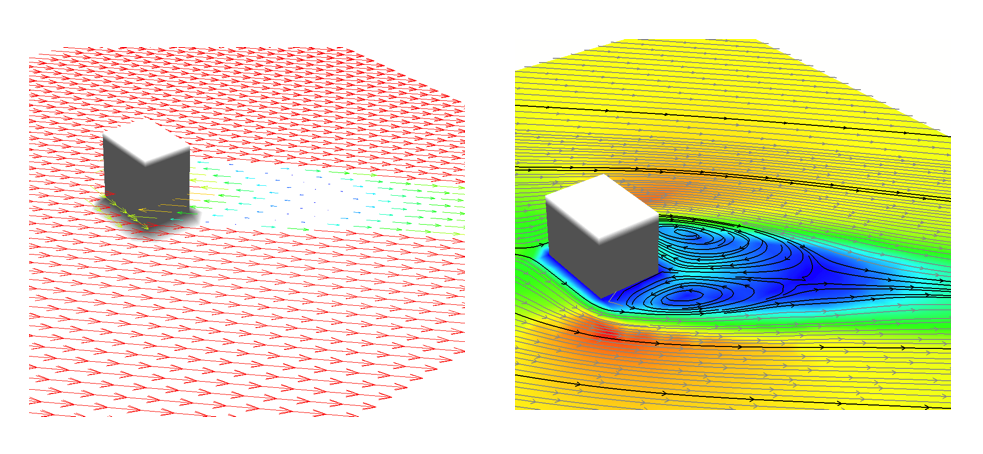
\includegraphics[width=0.75\textwidth]{swift_exemple}
	\caption{Exemple de calcul d'un champ de vent autour d'un obstacle avec SWIFT, avant (à gauche) et après (à droite) l'ajustement du champ}
	\label{fig_swift_exemple}
\end{figure}
En sortie de cet enchaînement de calculs, on obtient un champ de vent 3D qui peut alors directement être exploité par le modèle de dispersion SPRAY.



\subsubsection{SPRAY}

SPRAY est un modèle de dispersion lagrangien stochastique dont les principes de base suivent les mécanismes présentés à la section \ref{part_lagrangian}. L'implémentation de SPRAY repose sur le critère dit de \textit{well-mixed condition} permettant de donner une formulation explicite aux termes $a_i$ et $b_{i,j}$ de l'équation \eqref{eq_langevin} , et présenté en détail dans les travaux de \cite{Thomson1987}.

En pratique, plusieurs fonctionnalités supplémentaires sont implémentées dans SPRAY, telles que: \\

\begin{itemize}
	\item le "rebond" des particules sur les obstacles,
	\item le calcul de doses pour les sources radioactives,
	\item la prise en compte des différents types de dépôts (secs ou humides).\\
\end{itemize}

\begin{figure}[h!]
	\centering
	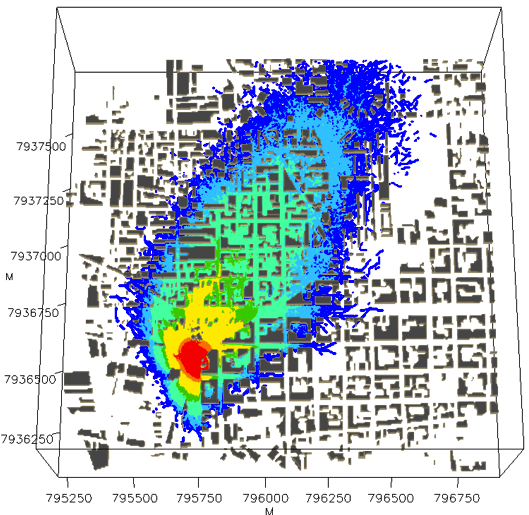
\includegraphics[width=0.65\textwidth]{spray_exemple}
	\caption{Exemple de champ de concentration calculé par SPRAY dans un domaine de type urbain}
	\label{fig_spray_exemple}
\end{figure}

La combinaison de SWIFT et SPRAY permet ainsi de calculer un champ de concentration sur le domaine étudié, connaissant les paramètres du terme source qui sont soumis en entrée du modèle SPRAY. Dans ce chapitre, la chaîne de calcul PMSS est utilisée à a fois pour : \\

\begin{itemize}
	\item simuler un rejet induit par une source que l'on va chercher à retrouver: pour cela, on va récupérer les valeurs de concentration sur un nombre fini de points du domaine que nous définirons comme étant les valeurs d'observation fournies par les capteurs,
	\item à construire les matrices source-récepteur nécessaires au processus d'estimation du terme source.\\
\end{itemize}

Sur ce dernier point, comme il s'agit désormais de travailler avec un outil de simulation relativement complet, et nécessitant \textit{de facto} des temps de calculs plus importants, il devient nécessaire d'optimiser le schéma algorithmique de l'estimation des paramètres de la source. Nous détaillons l'approche choisie dans la partie suivante.


\subsection{Dualité \textit{forward-backward}}

L'optimisation du calcul des matrices source-récepteur suivant le modèle de l'équation \eqref{eq_AE_4} est un point important: en effet dans une approche directe telle que présentée dans le chapitre précédent, la construction des $\MatC(\VecTheta)$ pour chaque particule $\VecTheta$ échantillonnée depuis la loi de proposition courante fait appel à autant de calculs de dispersion, ce qui rend l'opération d'estimation du terme source très coûteuse en temps de calcul.\\

Nous proposons ici une amélioration du processus d'estimation privilégiant le calcul des matrices source-récepteur par une approche de type \textit{backward}, reposant sur l'utilisation d'un modèle de dispersion adjoint. Cette méthodologie a initialement été introduite dans \cite{Keats2007} pour ensuite être appliquée sur un algorithme d'estimation de type MCMC.

Soit une source ponctuelle $Q$ située au point de l'espace $\PosSource$, de débit massique constant $q_s$ et de temps d'activation et d'arrêt respectifs $t_{on}$ et $t_{off}$ définie par la distribution suivante:\\

\begin{equation}
	Q = q_s \delta(\Vecx - \PosSource)\left[H(t - t_{on}) - H(t - t_{off})\right]
\end{equation}
où $\delta$ est la distribution de Dirac et $H$ la fonction de Heaviside. On note $C$ le champ de concentration moyen induit par cette  source. La valeur simulée de concentration $c_i$ obtenue sur le $i$-ème capteur à l'instant $t$ peut se modéliser par l'équation suivante:

\begin{equation}
c_i = \int_0^t \int_V C h ~dtdV
\label{eq_int_direct}
\end{equation}
où $h$ est la \textit{fonction} de réponse du capteur. Cette équation peut se simplifier sous la notation suivante:\\

\begin{equation}
c_i = \langle	C,h\rangle
\label{eq_scal_direct}
\end{equation} 

La relation de \textit{dualité forward-backward} présentée par \cite{Keats2007} stipule que cette même concentration peut s'écrire sous la forme:

\begin{equation}
c_i = \int_0^t \int_V Q C^* ~ dtdV = \langle Q, C^*\rangle
\label{eq_int_adjoint}
\end{equation}
où $C^*$ est le champ de rétro-concentrations induit par le $i$-ème capteur, et dont les valeurs sont obtenues par la résolution de l'équation \eqref{eqn_advection_diffusion_backward}. Dans la pratique, le champ $C^*$ est simulé par un \textit{modèle de dispersion adjoint}.

La relation de dualité $\langle C,h\rangle = \langle Q,C^* \rangle$ est ainsi valable si l'équation adjointe d'advection-diffusion a été résolue de telle sorte que les conditions aux limites permettent d'annuler les termes de bord pouvant y apparaître. De plus:

\begin{enumerate}
	\item sous l'hypothèse d'un capteur idéal, sa résolution est infinie, ce qui se traduit en pratique par $h$ prenant la forme d'une distribution de Dirac,
	\item dans le cadre de la construction des matrices source-récepteur, $Q$ illustre une source instantanée et dont le débit de rejet est unitaire.
\end{enumerate}

Dans ce cas particulier, on obtient alors une équivalence entre $C$ et $C^*$: 

\begin{equation}
C \simeq C^*
\label{eq_equivalence}
\end{equation}

En pratique, l'égalité n'est pas stricte du fait de l'erreur des modèles directs et adjoints à partir desquels sont obtenus les deux champs, mais les valeurs sont relativement proches. \\

Le fait de substituer un modèle adjoint au modèle direct permet de n'avoir à faire qu'un seul calcul de dispersion par capteur, qui donne alors l'ensemble des valeurs de rétro-concentrations sur le domaine. On peut alors réutiliser ces valeurs à chaque itération de l'algorithme AMIS, au lieu de relancer une série de calculs en mode \textit{forward}. En pratique, à paramètres identiques une simulation en \textit{forward} est aussi longue qu'en \textit{backward}, mais le gain en temps de calcul s'illustre par le fait de sortir cette simulation \textit{backward} du schéma itératif de l'algorithme d'estimation.



\subsection{Intégration de RetroSPRAY au processus d'estimation}

\subsubsection{Principe théorique}

Il nous est possible d'avoir recours au calcul des rétro-concentrations grâce à l'existence d'un modèle de dispersion adjoint appelé RetroSPRAY, associé à la suite de calcul PMSS. Ce dernier procède à la résolution des équations de Langevin en mode inverse: en prenant en compte un pas de temps positif, on a: 

\begin{equation}
\begin{split}
du_i^b &= U_i^b (t-dt) - U_i^b(t) \\
dx_i^b &= x_i^b (t-dt) - x_i^b(t)
\end{split}
\label{eq_langevin_inv1}
\end{equation}

On peut alors écrire l'équivalent inverse de l'équation \eqref{eq_langevin} sous la forme suivante:

\begin{equation}
	\begin{split}
	du_i^b &= a_i^b dt + b_{i,j}^b d\xi_j \\
	dx_i^b &= -(\bar{u}_i + U_i^b )dt
	\end{split}
	\label{eq_langevin_inv2}
\end{equation}

Les termes $a_i^b$ et $ b_{i,j}^b$ peuvent être calculés selon les expressions fournies dans \cite{Flesch1995} et \cite{Wilson2009}. \\

Si on examine plus en détail la construction de la matrice source-récepteur, on peut réécrire l'équation \eqref{eq_AE_4} sous une forme plus explicite: notons $C(R_i,t_j |\VecTheta, t'_n)$ la concentration moyenne au capteur $R_i$ à l'instant $t_j$ résultant d'une source située à la position $\VecTheta$ et ayant émis un rejet unitaire à l'instant $t'_n$. La version \textit{forward} de la matrice source-récepteur pour $\VecTheta$ s'écrit:

\begin{equation}
\MatC^f(\VecTheta) = 
\begin{pmatrix}
C(R_1,t_1 | \VecTheta, t'_1) & C(R_1,t_1 | \VecTheta, t'_2) & \cdots & C(R_1, t_1 |\VecTheta, t'_{T_s}) \\
C(R_1,t_2 | \VecTheta, t'_1) & C(R_1,t_2 | \VecTheta, t'_2) & \cdots & C(R_1, t_2 |\VecTheta, t'_{T_s}) \\
\vdots & \vdots & & \vdots \\
C(R_1,t_{T_c} | \VecTheta, t'_1) & C(R_1,t_{T_c} | \VecTheta, t'_2) & \cdots & C(R_1, t_{T_c} |\VecTheta, t'_{T_s}) \\
C(R_2,t_1| \VecTheta, t'_1) & C(R_2,t_1 | \VecTheta, t'_2) & \cdots & C(R_2, t_1 |\VecTheta, t'_{T_s}) \\
\vdots & \vdots & & \vdots \\
\vdots & \vdots & & \vdots \\
C(R_{N_c},t_{T_c} | \VecTheta, t'_1) & C(R_{N_c},t_{T_c} | \VecTheta, t'_2) & \cdots & C(R_{N_c}, t_{T_c} |\VecTheta, t'_{T_s}) \\
\end{pmatrix}
\label{eq_matrix_forward}
\end{equation}

En appliquant la relation de dualité \textit{forward-backward}, dans l'espace dual où le modèle adjoint opère, les sources deviennent des "rétro-capteurs", et les capteurs deviennent des "rétro-sources". On définit alors $C^*(\VecTheta,t'_n | R_i, t_j)$ comme la rétro-concentration mesurée au point $\VecTheta$ à l'instant $t'_n$ provenant d'une rétro-source située à la position $R_i$ et ayant émis un rétro-rejet unitaire à l'instant $t_j$. La version \textit{backward} de $\MatC^f$ s'écrit alors:

\begin{equation}
\begin{pmatrix}
\MatC^b (\VecTheta)= 
	C^*(\VecTheta, t'_1 | R_1, t_1) & C^*(\VecTheta, t'_2 | R_1, t_1) & \cdots & C^*(\VecTheta, t'_{T_s} | R_1, t_1) \\
	C^*(\VecTheta, t'_1 | R_1, t_2) & C^*(\VecTheta, t'_2 | R_1, t_2) & \cdots & C^*(\VecTheta, t'_{T_s} | R_1, t_1) \\
	\vdots & \vdots & & \vdots \\
	C^*(\VecTheta, t'_1| R_1,t_{T_c}) & C^*(\VecTheta, t'_2 | R_1, t_{T_c}) & \cdots & C^*(\VecTheta, t'_{T_s} | R_1, t_{T_c}) \\ 
	\vdots & \vdots & & \vdots \\
	\vdots & \vdots & & \vdots \\
	C^*(\VecTheta, t'_1| R_{N_c},t_{T_c}) & C^*(\VecTheta, t'_2 | R_{N_c}, t_{T_c}) & \cdots & C^*(\VecTheta, t'_{T_s} | R_{N_c}, t_{T_c}) \\ 
	
\end{pmatrix}
\label{eq_matrix_backward}
\end{equation}

Il s'agira donc de privilégier $\MatC^b$ lors des applications pratiques, au moment de modéliser les concentrations comme il est fait  à l'équation \eqref{eq_AE_2} par exemple. Les tests préliminaires qui ont été effectués ont pu montrer l'équivalence entre les deux formulations matricielles, comme illustré à la figure \ref{fig_comparaison_matrices}.

\begin{figure}[h!]
	\centering
	\begin{subfigure}[t]{0.5\textwidth}
		\centering
		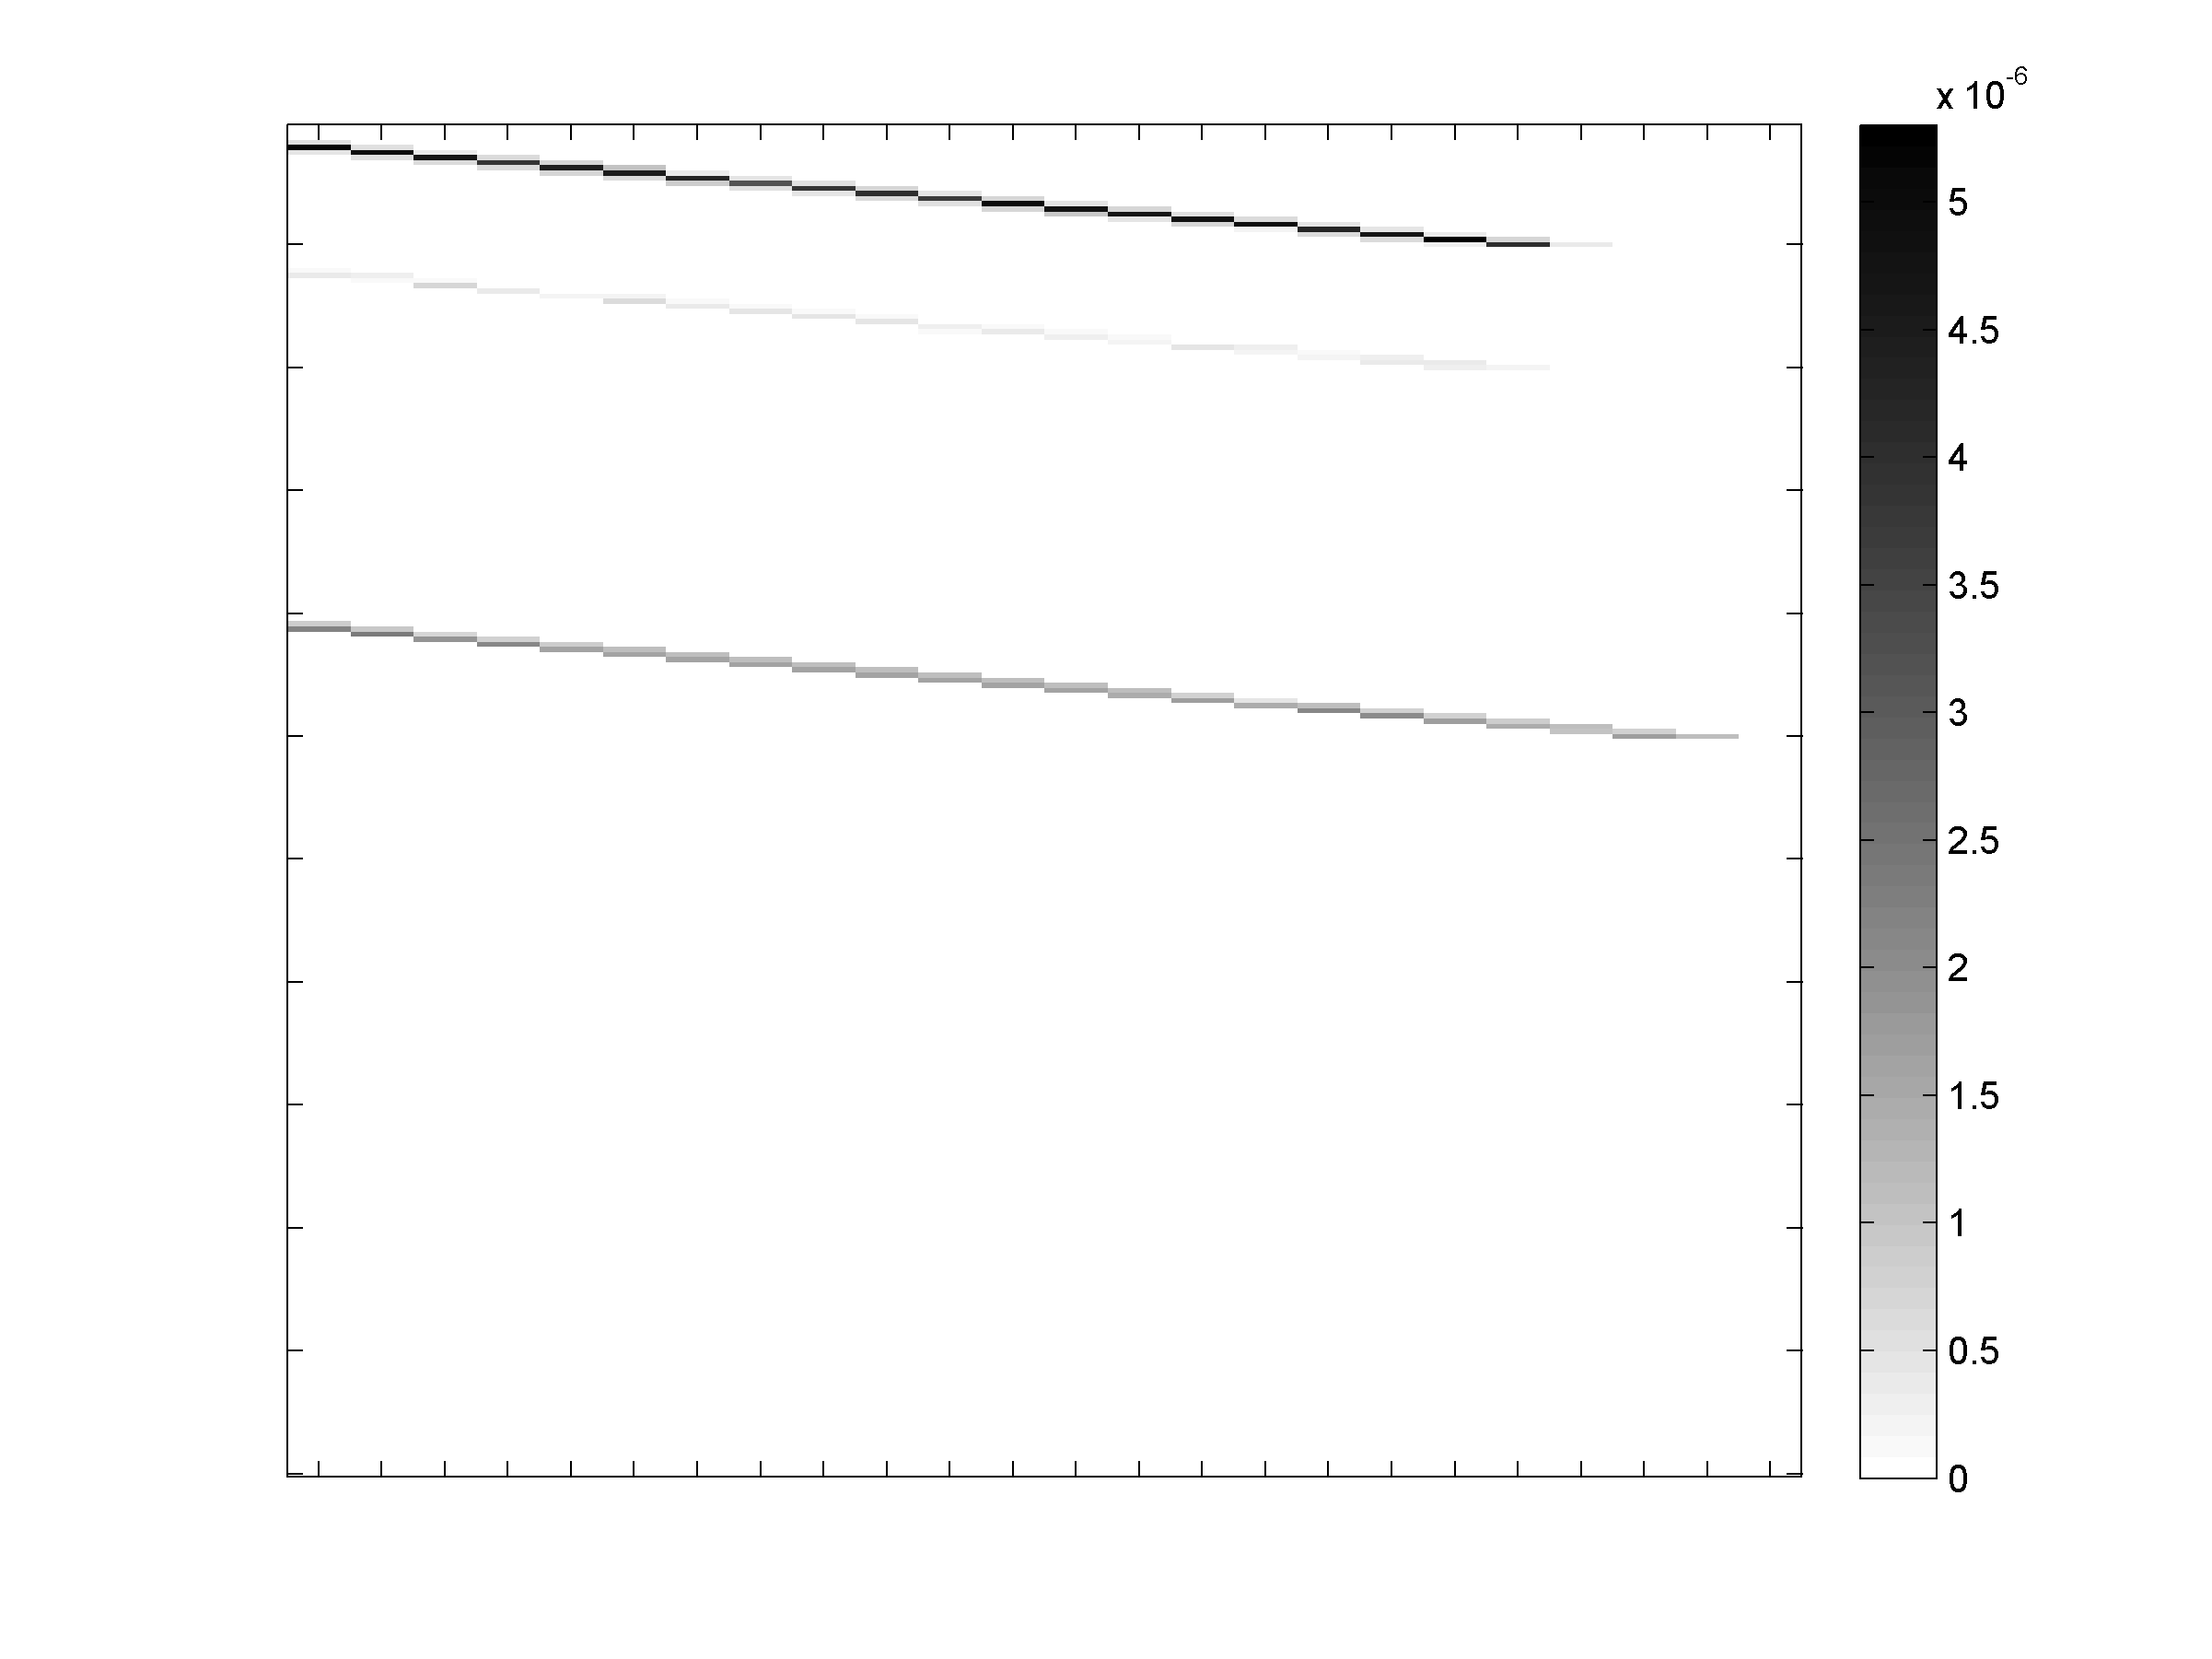
\includegraphics[width=1\textwidth]{m_forward}
		\caption{}
		\label{forward}
	\end{subfigure}%
	\begin{subfigure}[t]{0.5\textwidth}
		\centering
		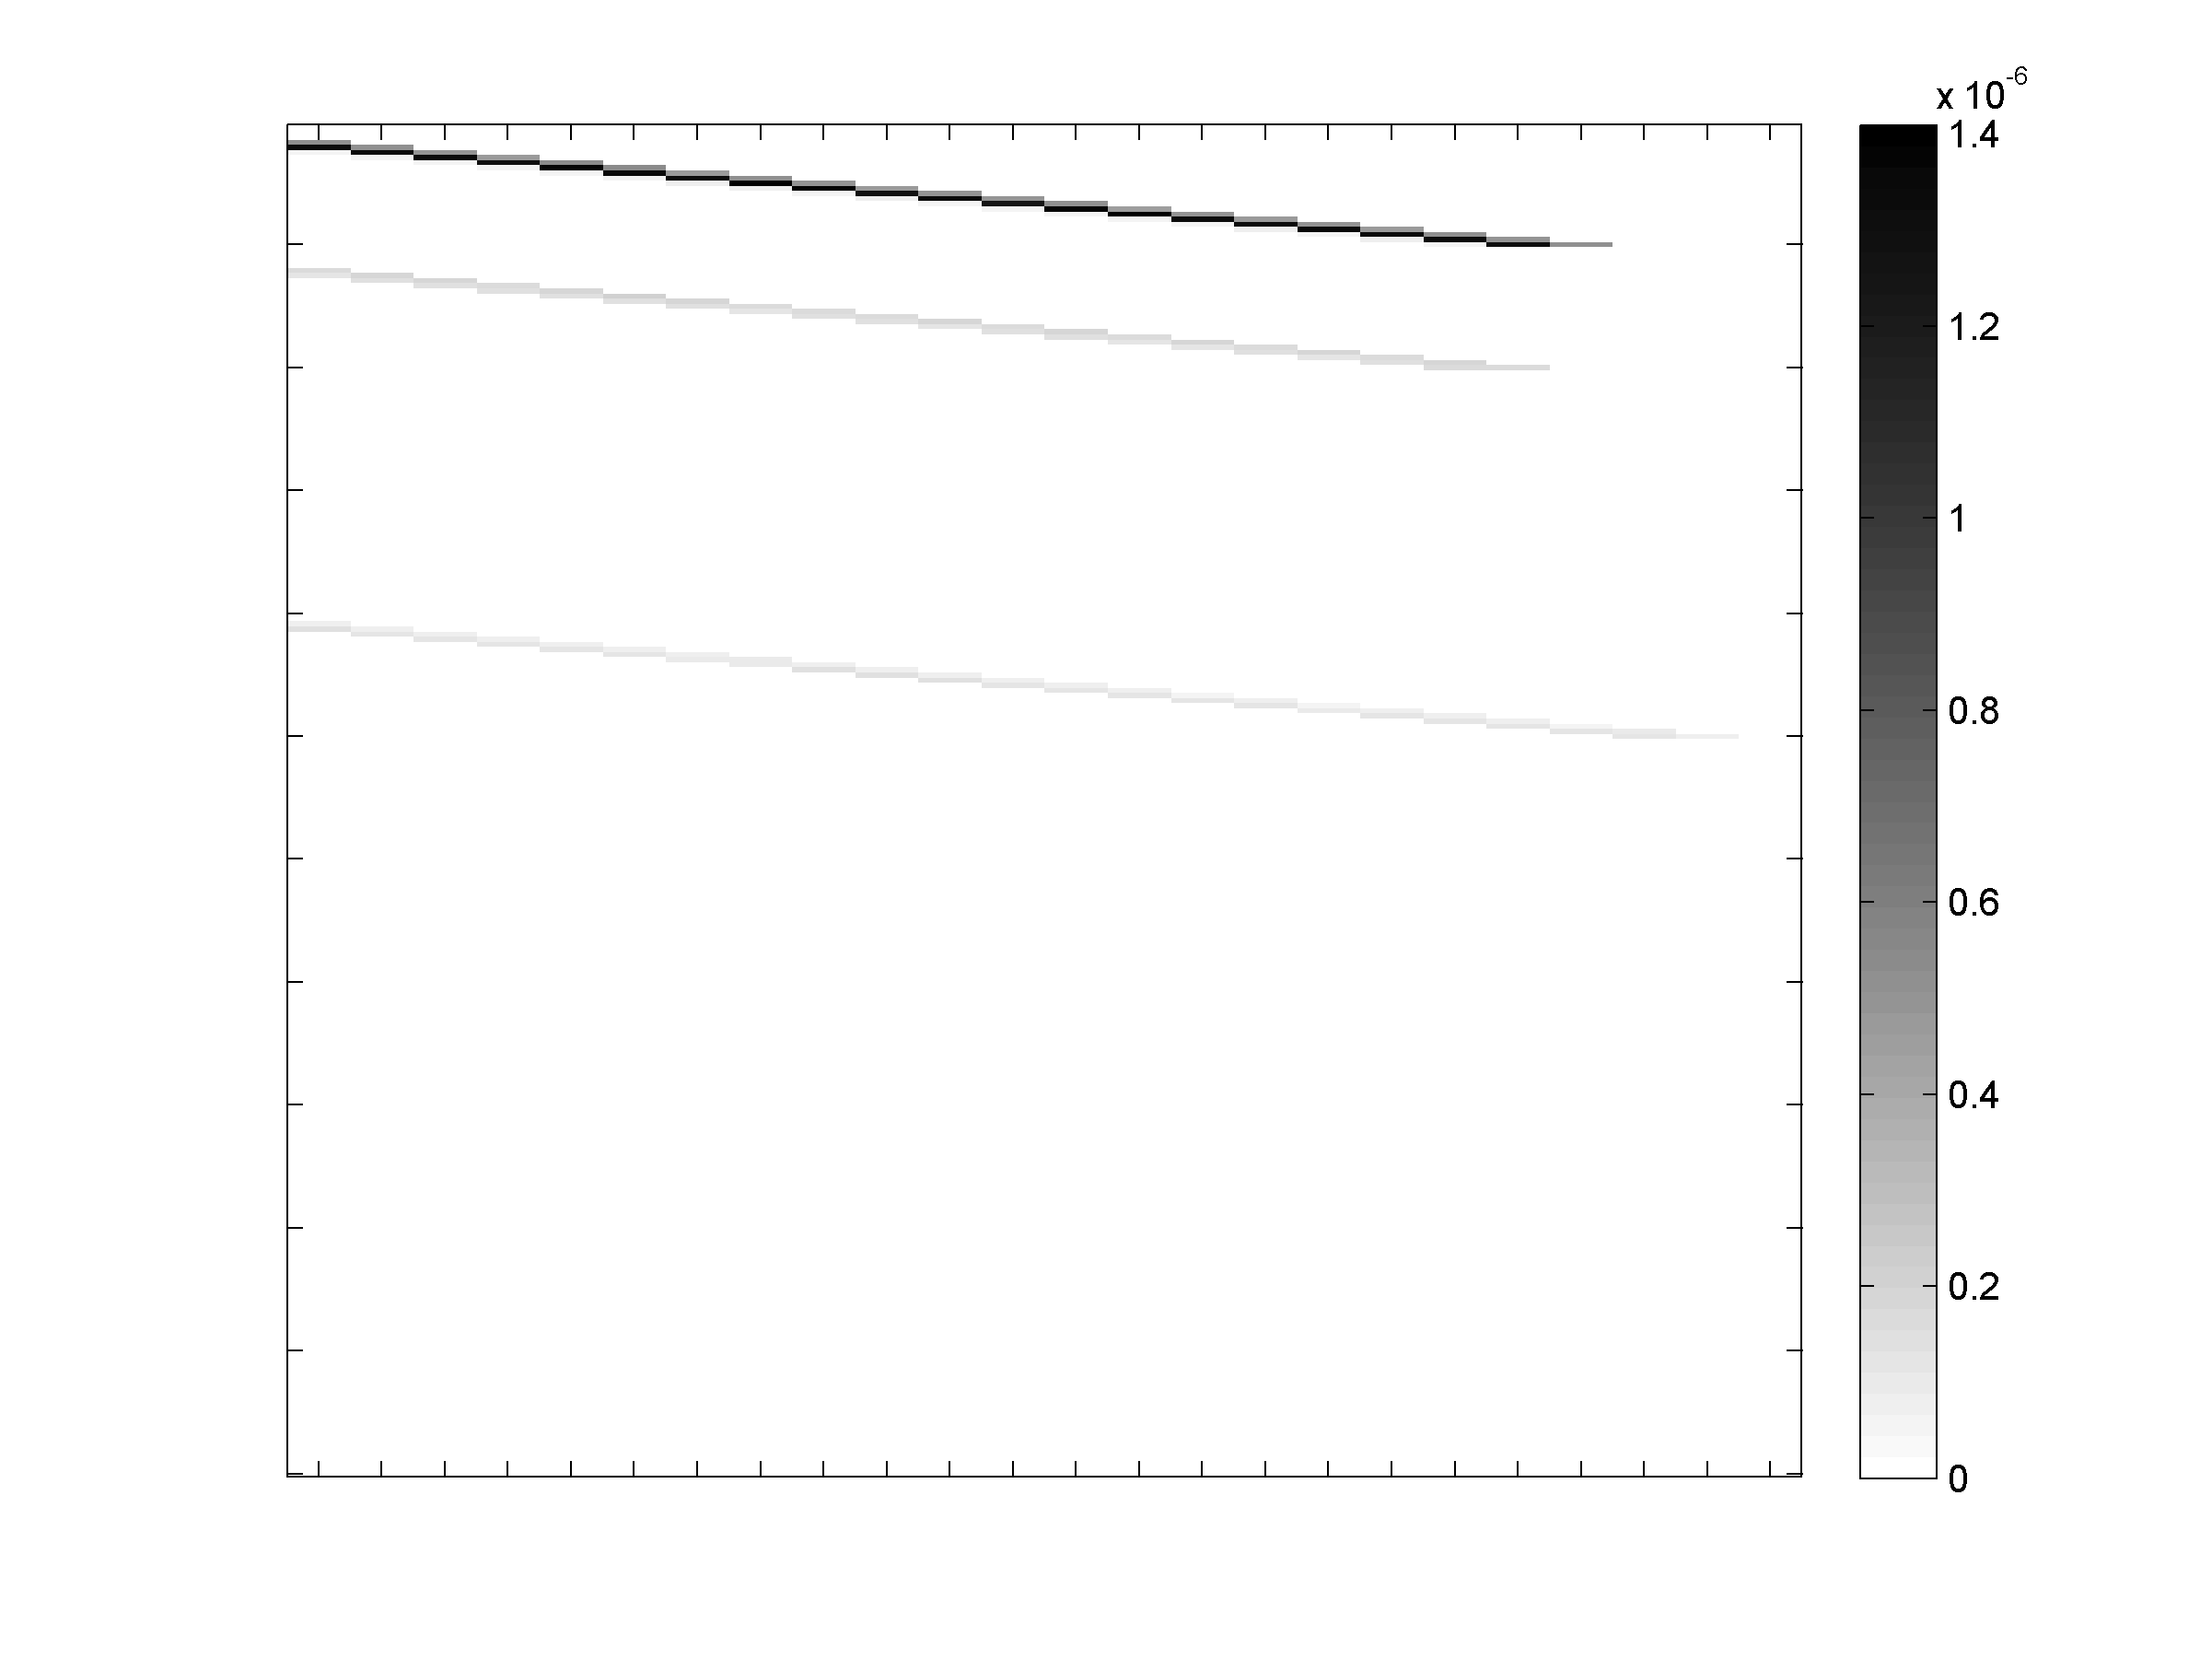
\includegraphics[width=1\textwidth]{m_backward}
		\caption{}
		\label{backward}
	\end{subfigure}
	\caption{Comparaison des matrices source-récepteur obtenues pour une source instantanée ayant émis un rejet unitaire: avec un calcul \textit{forward} (à gauche) et un calcul \textit{backward} (à droite)}
	\label{fig_comparaison_matrices}	
\end{figure}

\subsubsection{Implémentation}

Concrètement, l'utilisation de RetroSPRAY implique un transfert de la charge de calcul liée à l'exécution du modèle de dispersion en dehors du schéma itératif de l'AMIS. Avant tout calcul d'estimation, un ensemble de fichiers binaires contenant les différents champs de rétro-concentration sur tout le domaine est créé au cours d'une étape de pré-calcul. 

Ainsi, durant le processus d'estimation, au moment de construire les matrices source-récepteur à partir des particules fournies par le tirage depuis la loi de proposition, au lieu d'envoyer les positions vers le modèle de dispersion \textit{forward} celles-ci sont redirigées vers une fonction dont le rôle est de renvoyer directement en mémoire les valeurs de $C^*$ nécessaires après lecture des fichiers binaires. Comme le montre la figure \ref{fig_schema_amis_optimise}, aucun calcul de dispersion à proprement parler n'est alors effectué dans le schéma itératif, seulement une série d'opérations de lecture de fichiers.\\

\begin{figure}[h!]
	\centering
	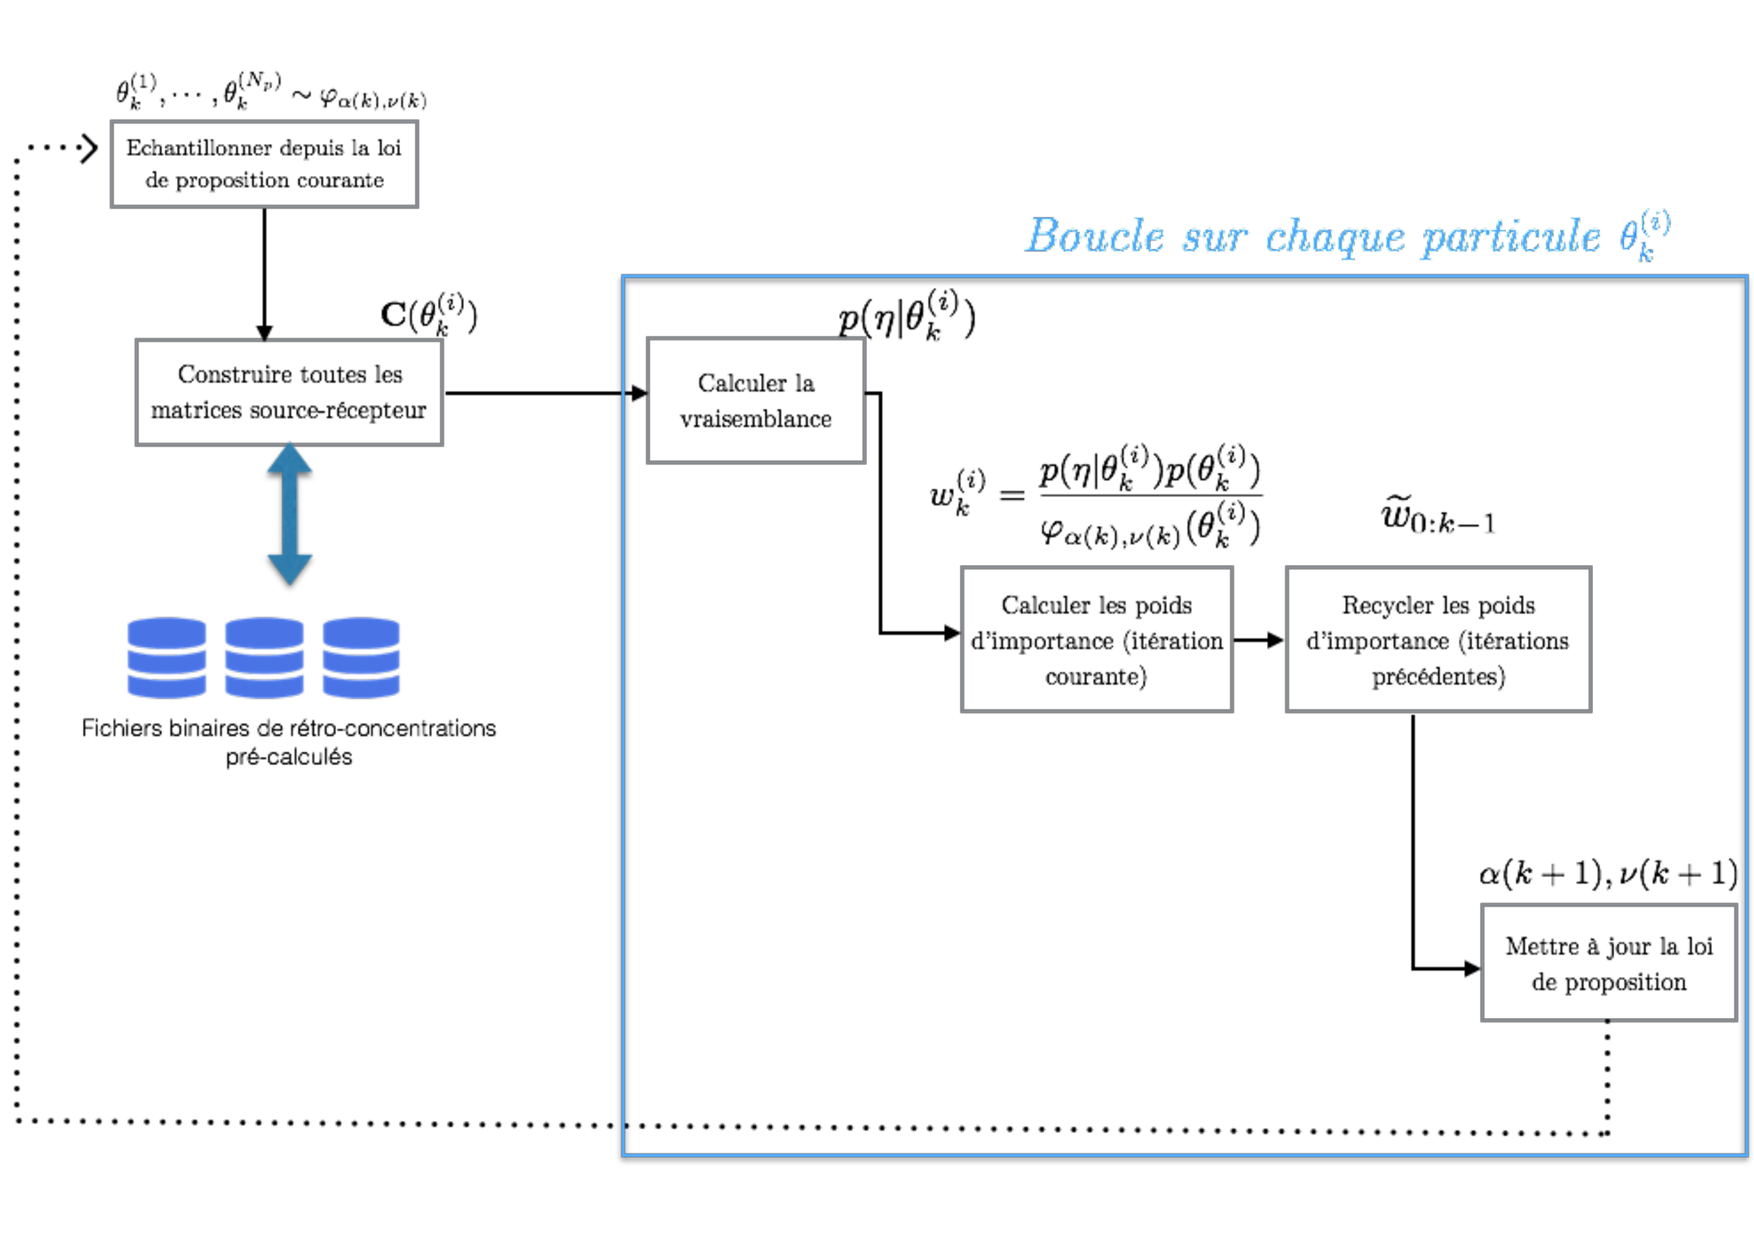
\includegraphics[width=0.75\textwidth]{schema_amis_optimise}
	\label{fig_schema_amis_optimise}
	\end{figure}
	
Dans les paragraphes suivants nous illustrons la mise en pratique de ce système optimisé sur plusieurs cas-tests simulés. \\



\section{Exemple d'application en rase campagne}

Dans cette section nous présentons un première application sur une situation  simple dans un contexte non-urbain.

\subsection{Présentation du cas-test}

Nous considérons ici un cas-test en milieu rural de moyenne échelle reproduisant une émission accidentelle dans une zone située près de la commune de Beaune, en Bourgogne, en présence d'une topographie réelle. 

\begin{figure}[h!]
	\centering
	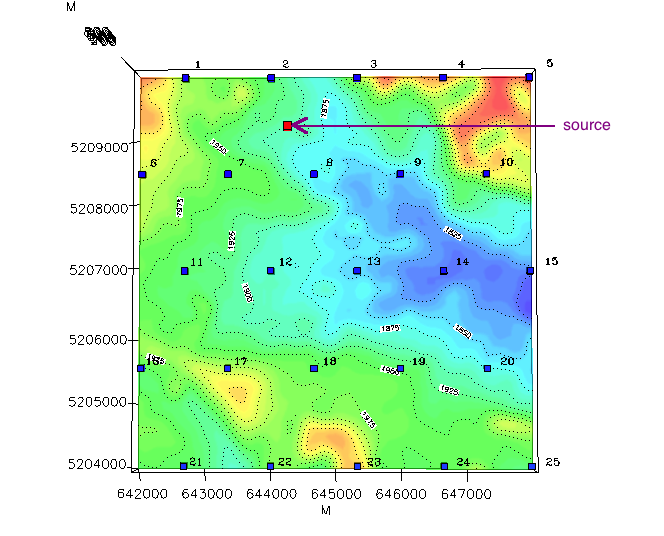
\includegraphics[width=0.7\textwidth]{beaune_relief_capteurs}
	\caption{Superposition du relief, de l'emplacement des capteurs et de la source du cas-test Beaune}
	\label{fig_beaune_relief}
\end{figure}

\subsubsection{Caractéristiques du domaine}
Le domaine considéré est une surface carrée de $6 \text{km}^2$, avec une source unique et un réseau relativement dense de 25 capteurs disposés en quinconce et couvrant toute la superficie du domaine (figure \ref{fig_beaune_relief}).

Pour la simulation utilisant l'outil PMSS, le domaine est discrétisé en une grille de $300 \times 300$ mailles, avec une résolution du maillage en $x$ et $y$ de $20\text{m}$. 

\subsubsection{Paramètres météorologiques}
Sur toute la durée de la simulation, nous considérons un vent constant en vitesse ($1.5\text{m/s}$) et en direction ($330\degres$). Cela produit un champ de vent relativement homogène (figure \ref{fig_beaune_vent}).

\begin{figure}[h!]
	\centering
	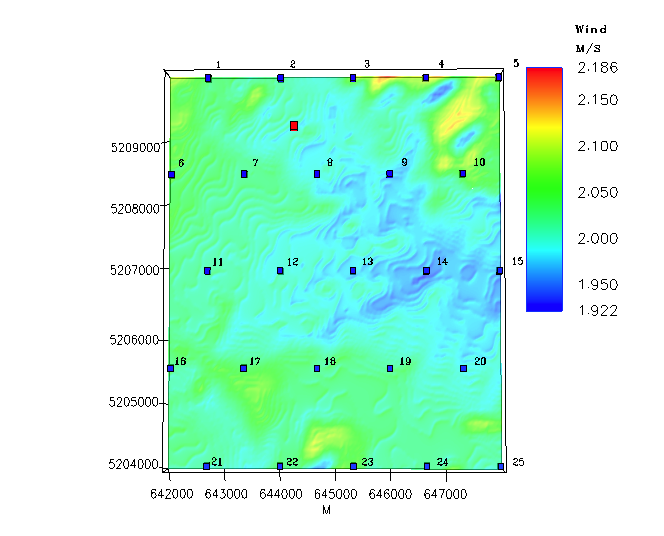
\includegraphics[width=0.7\textwidth]{beaune_vent}
	\caption{Champ de vent calculé par SWIFT pour le cas-test Beaune}
	\label{fig_beaune_vent}
\end{figure}


\subsubsection{Paramètres relatifs à la source}
Afin de simuler les observations aux capteurs, on choisit une source unique située dans la partie nord (voir figure \ref{fig_beaune_relief}) afin que le panache résultant couvre une partie suffisante du domaine. La source est située à une altitude de 10m, et émet un rejet unique entre 10h15 et 11h, avec un débit constant de 1850 unités/s. Pour la simulation, cette source est modélisée comme étant un volume de 15m $\times$ 15m $\times$ 10m. \\

\begin{figure}[h!]
	\centering
	\begin{subfigure}[t]{0.5\textwidth}
		\centering
		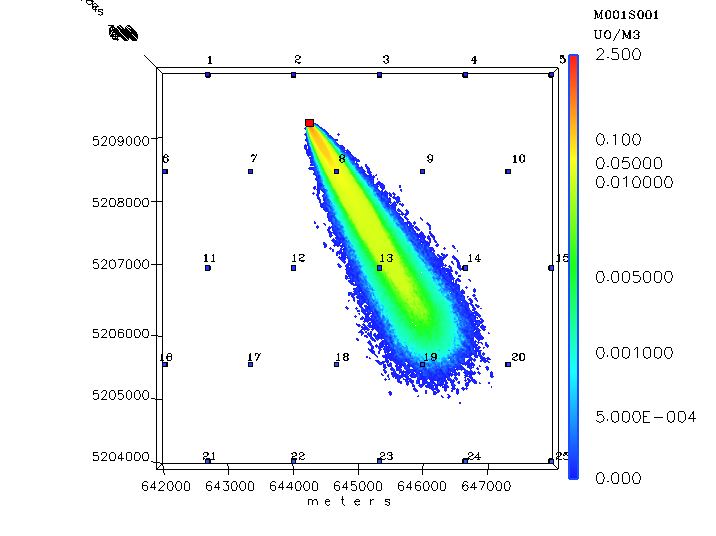
\includegraphics[width=1\textwidth]{source_1_12}
		\caption{Instantané du panache à 10h55}
		\label{panache}
	\end{subfigure}%
	\centering
	\begin{subfigure}[t]{0.5\textwidth}
		\centering
		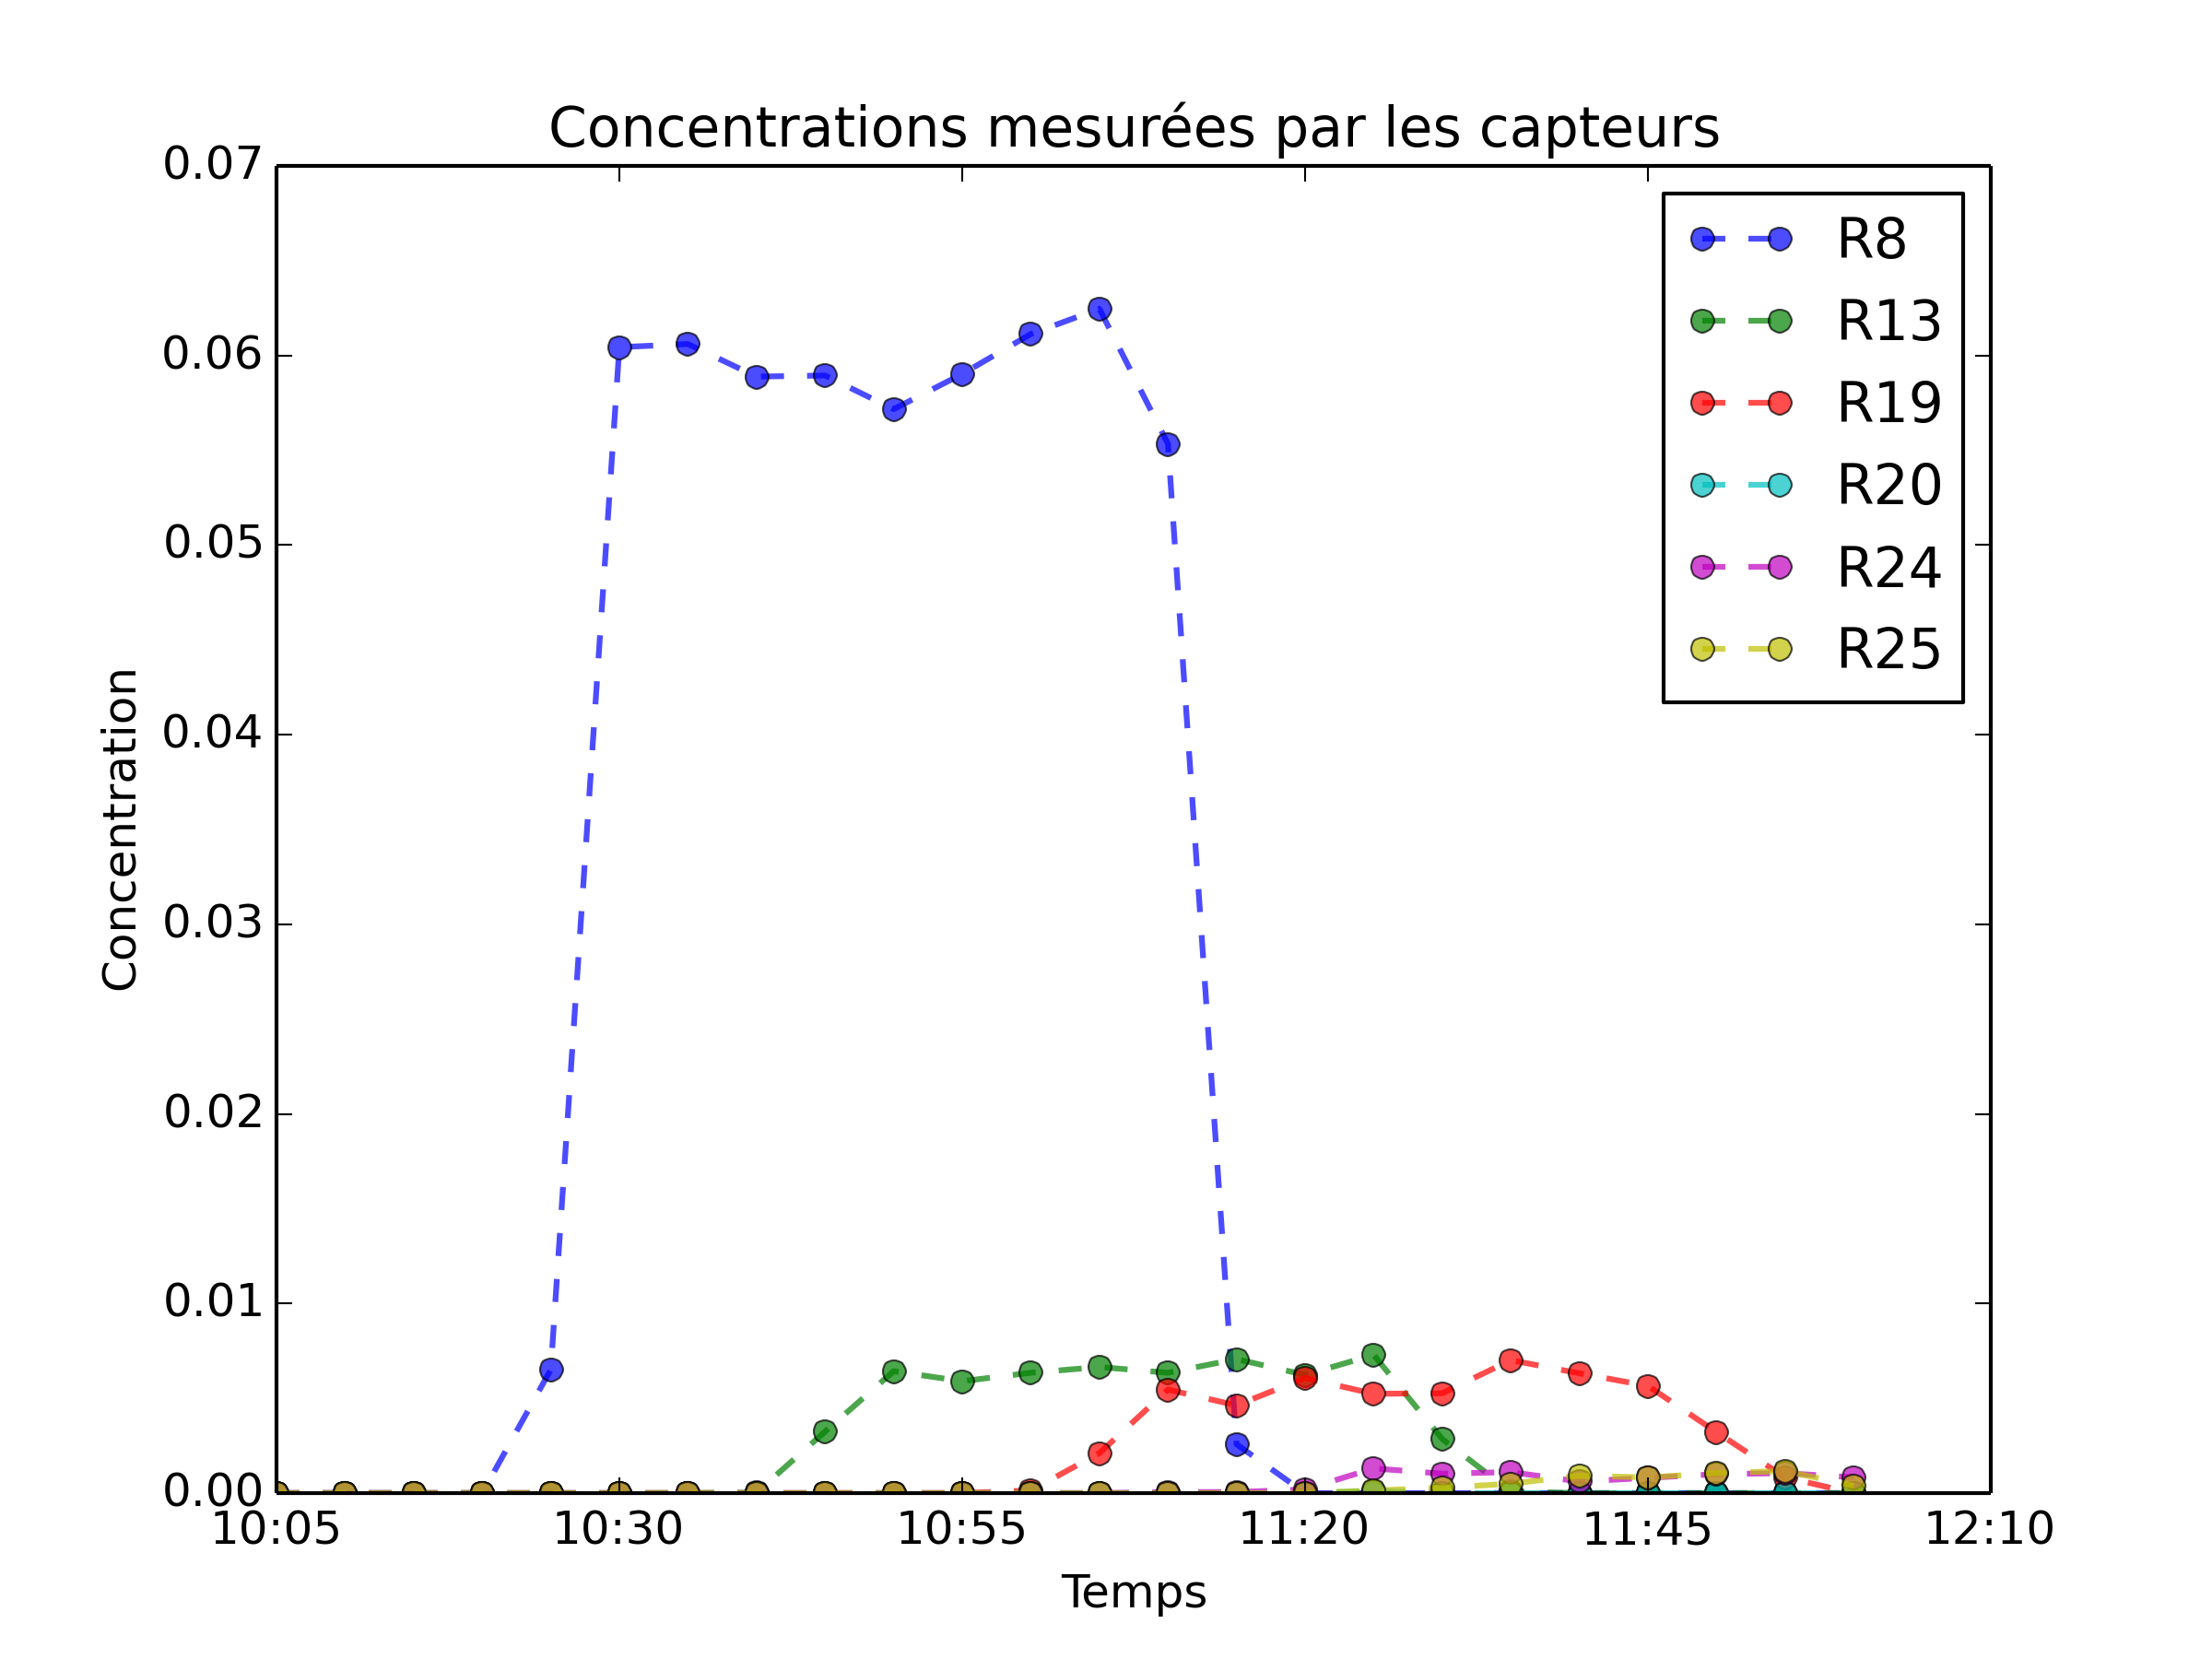
\includegraphics[width=1\textwidth]{obs_vent_330}
		\caption{Concentrations aux capteurs}
		\label{series_temporelles}
	\end{subfigure}
	\caption{Caractéristiques du rejet simulé: forme du panache (\ref{panache}) et concentrations moyennes aux capteurs impactés par le rejet (\ref{series_temporelles})}
	\label{fig_rejet_beaune} 
\end{figure}

\missingfigure{Remplacer figure \ref{fig_rejet_beaune} par snapshots à 6 instants sur 1 page.}

La figure \ref{panache} illustre l'allure du panache résultant de la source simulée par SPRAY, et sa propagation dans l'axe du vent. La figure \ref{series_temporelles} représente les séries temporelles de concentrations moyennes relevées aux capteurs impactés par le panache.

\subsubsection{Paramètres relatifs aux capteurs}
On considère un réseau de 25 capteurs disposés de façon à couvrir tout le domaine, et placés à une hauteur de 10m, égale à celle de la source. Chaque capteur est modélisé par un volume de 15m $\times$ 15m $\times$ 10m, et fournit des observations de concentrations moyennes entre 10h05 et 12h (voir figure \ref{series_temporelles}). La moyenne des concentrations s'effectue sur des plages de 5 minutes.

\missingfigure{Concentrations mesurées aux capteurs et constituant le vecteur d'observation utilisé en entrée de l'algorithme AMIS}

\subsubsection{Tableau récapitulatif}

\todoin{Faire un fat tableau récapitulant tous les paramètres précédemment énoncés}

\subsection{Analyse paramétrique sur $\varObs$}

\subsection{Analyse paramétrique sur $\varQ$}

\subsection{Modularité du réseau de capteurs}

\section{Exemple d'application à un cas urbain}

On considère à présent le cas d'un rejet bref dans un cadre urbain.\\

\subsection{Présentation du cas-test}

On se place à l'échelle d'un quartier, en l'occurrence celui de la Place de l'Opéra, à Paris: il s'agit ici d'une situation plus complexe par rapport au cas précédent, à cause de la présence d'obstacles multiples et de géométries variées sur le domaine (bâtiments). \\

\missingfigure{Opéra: domaine et capteurs}

\subsubsection{Caractéristiques du domaine}

On se place sur un domaine de 808m $\times$ 882m, soit environ $844\text{m}^2$. La discrétisation choisie est plus fine que dans le cas précédent, car la topographie est plus complexe: le domaine est ainsi divisé en 404 mailles selon $x$ et 441 mailles selon $y$, avec une résolution de 2m sur chaque direction. \\

\missingfigure{Schéma du domaine avec mise en évidence de l'aspect 3D}

\subsubsection{Paramètres météorologiques}

On choisit un vent de vitesse constante (3m/s) mais dont la direction change toutes les heures : \\

\begin{center}
\begin{tabular}{cccc}
	\centering
	Heure & 11:00:00 &  12:00:00 &  13:00:00\\ 
	\hline
	 Direction vent & $230\degres$ & $180\degres$ & $45\degres$
\end{tabular} 
\end{center}

La combinaison de ces variations temporelles ainsi que de la présence d'obstacles sur le domaine fait que les champs de vent 3D diagnostiqués par SWIFT sont relativement complexes, comme l'atteste la figure FIG.

\missingfigure{Champs de vent à 2m }

\subsubsection{Paramètres relatifs à la source}

On se place dans le cas d'une source unique située à 2m du sol, et qui émet un rejet bref d'une durée de 10 minutes entre 12h10 et 12h20, avec un débit constant de $10^4$ unités/s. Dans la simulation, cette source est modélisée par un volume de 4M $\times$ 4m $\times$ 2m. Ces caractéristiques se rapprochent de celles d'un rejet d'origine malveillante, par exemple suite à l'explosion d'une "bombe sale". \\

\missingfigure{Illustration du rejet 12h15 --> 12h40}

\subsubsection{Paramètres relatifs aux capteurs}

Le domaine contient un réseau de 10 capteurs, qui sont placés aux centres de diverses intersections de rues, ainsi que sur des places publiques. Ils sont situés à la même hauteur que la source, et leur volume de contrôle est de 4m $\times$ 4m $\times$ 2m. Ils délivrent des valeurs de concentrations moyennées sur des plages de 5 minutes. \\

\subsubsection{Tableau récapitulatif}




\subsection{Initialisation optimisée de la loi de proposition}

Dans une situation complexe comme celle du cas Opéra, il peut se révéler utile d'initialiser la loi de proposition pour l'AMIS de façon plus judicieuse qu'une simple hypothèse de répartition uniforme des particules sur le domaine. Une initialisation optimisée permettra ainsi d'explorer des zones potentiellement intéressantes plus rapidement, augmentant l'efficacité de l'algorithme d'estimation. \\

Comme dans notre cas on a choisi une loi de proposition de type mixture de $D$ gaussiennes $\varphi_1, \dots, \varphi_D$, on va chercher à estimer les moyennes $\left(\VecMu_d\right)_{1:d}$ et les matrices de covariance $\left(\MatSigma_d\right)_{1:d}$ de chacune de ces composantes, ainsi que leurs facteurs d'influence $\left(\alpha_d\right)_{1:d}$. 

Pour cela, in utilise les résultats issus d'un \textit{run} de rétro-propagation: suivant un modèle de dispersion adjoint, on construit une série de cartes des concentrations conjuguées sur tout le domaine, en transformant les capteurs en rétro-sources et en utilisant les concentrations mesurées comme valeurs de rétro-émission. Une fois ces cartes créées, elles sont vues comme des ébauches des densités de probabilité sur la position de la source pour différents temps d'émission. L'objectif est alors de caler les paramètres $\left(\alpha_d, \VecMu_d,\MatSigma_d \right)_{1:D}$ sur ces densités.\\

On part de l'instant d'observation $t_0$ qui est celui où la concentration la plus élevée a été observée. On définit ensuite un instant $t_{RP}$ qui correspond à l'instant final de la rétro-propagation, avec $t_{RP} < t_0$. 

\subsection{Résultats}





